\section{An introduction to Whole-body control}\label{wbp:sec:intro}
Over the past years, increasing research attention has been devoted to domestic service robots. These robots usually consist of a mobile base with one or two robotic arms. These arms have six or seven Degrees-of-Freedom (\dofs) and are commonly mounted on a torso with additional \dofs. A fundamental competence of these robots is the ability to safely manipulate objects in a domestic environment.

% Whole-body controller
Many of the control methods for this purpose are based on the operational space formulation~\citep{Khatib1987}. This formulation eventually resulted in whole-body control, of which implementations can be found in, \eg, \citet{Nagasaka2010,Dietrich2012} and \citet{Gienger2005,Sentis2005}, where the latter references concern biped humanoid robots instead of wheeled mobile robots.
There are various motives that justify the use of whole-body controllers in a domestic environment:
\begin{itemize}
    \item Robustness against dynamic environments due to the presence of humans. This requires reactive motions, which is a key feature of whole-body controllers. 
    A task of a whole-body controller is typically defined as an impedance in \emph{Cartesian space}, \ie, as a virtual spring between the current end-effector pose and the desired end-effector pose (also called `attractor'). By defining this as a compliant spring rather than a stiff trajectory, tasks involving interaction with the environment are more robust against inaccuracies in the environment model and this compliance enhances safety in case of undesired interaction with the environment.
%    As a result, the arm can deviate from its trajectory in case of undesired interaction with the environment, enhancing safety.
    \item the kinematic redundancy of domestic service robots. Both the path and goal constraints of a task are typically defined in Cartesian space, and due to this redundancy the specification of joint positions and trajectories is no longer a practical means of defining a task~\citep{Brock2002a}. This is especially true if a robot has multiple manipulators. In whole-body control, the redundancy is utilized for online optimization of secondary motion objectives such as keeping a desired posture and avoiding joint limits.
%    \item A whole-body controller typically results in predictable robot motions since the end-effector is drawn towards its goal pose in Cartesian space.
	\item Since the end-effectors are controlled in Cartesian space, a point-to-point motion typically results in an end-effector trajectory that is straight in Cartesian space, which looks much more human-like than a trajectory that is straight in joint space.
\end{itemize}

% Needs planner
% -- req1: global scope
However, since whole-body control is a potential field based method, it only operates at a local scope. As a result, it might be unable to find a global solution in a complex environment with local minima. This illustrates the need for a global planning method on top of the whole-body controller, as is recognized by, \eg, \citet{Yang2006,Toussaint2007,Behnisch2010,Behnisch2011,Dietrich2012}.

% -- req2: minimize number of constrained DoFs
An important issue for this global planning method is the question which \dofs\ to constrain. 
Already in~\citet{Nakanishi2007}, it is argued that it is desirable to control only the minimum number of \dofs\ of a robot such that the remaining \dofs\ can be utilized to optimize secondary motion objectives in the null space of the primary task. %compliant redundancy resolution
The minimum number of \dofs\ required to complete a task may even vary during a motion. 
%These path constraints can vary during a certain motion: 
An example is grasping an object from a table. Initially, the end-effector moves to the correct height while being close to the robot to avoid the table (the height and distance to the robot body are constrained by the task), then moves to a pre-grasp pose and a grasp pose (up to six \dofs\ need to be constrained). After closing the gripper, the object is lifted (the height and possibly, to keep an object such as a coffee cup level, roll and pitch are constrained) and the arm is retracted (the end-effector needs to be close to the robot and roll and pitch are possibly constrained).

%Therefore, a planner is required that provides connectivity information on a global scope while minimizing the number of constrained \dofs.
%To integrate a whole-body controller in a task executer, a planner is required that provides connectivity information in a global scope while constraining only the \dofs\ that are relevant for the (sub-) task at hand.
To integrate a whole-body controller in a task executer, a planner is required that provides connectivity information in a global scope. Furthermore, it constrains only the \dofs\ that are relevant for the (sub-) task at hand to maximize the number of redundant \dofs\ that can subsequently be used to optimize secondary motion objectives.
% global scope, connectivity

\section{Related work and contribution}
In literature, examples can be found of motion planners that i) plan in joint space, ii) plan an end-effector path in Cartesian space, typically represented as a sequence of attractors or iii) call motion primitives from a task executer.

%Currently, many motion planners for manipulators plan in joint space. 
A recent example of a joint space planner can be found in~\citet{Sucan2012}. However, this planner does not take path constraints into account. To include path constraints when planning in the joint space, a constraint manifold is computed and a path is searched on that manifold~\citep{Sucan2012a}. 
%Although good results can be obtained with these planners, there is no robustness against dynamic environments: the increasing number of degrees of freedom increases computational complexity for motion planning in joint space and hence limits the ability to replan~\citep{Brock2002a}. 
Although good results can be obtained with these planners, there is no robustness against dynamic environments: the increasing number of degrees of freedom increases computational complexity for motion planning in joint space. For a \ndof{7}\ arm, planning times are in the order of magnitude of $0.5\ \mathrm{s}$ and these planning times will increase with increasing number of \dofs. This limits the ability to replan~\citep{Brock2002a}.
%Furthermore, planning in joint space may result in unpredictable motions in Cartesian space.
Furthermore, planning in joint space may result in motions that are far from human-like, which is undesired for anthropomorphic domestic robots.

For whole-body controllers, the planners do not result in an explicit trajectory but rather a sequence of attractors in Cartesian space. These attractors can constrain up to six \dofs\ of the end-effector, \ie, both the position and the orientation. 

In~\citet{Brock2002a}, the concept of elastic strips is introduced as a framework to robustly execute a global motion. However, it is not discussed how this global motion is computed or how to recover from an invalidation of the global motion. To include this global connectivity information, elastic roadmaps are introduced in~\citet{Yang2006,Yang2010}. Here, a sampling-based planning approach is used to create a roadmap in workspace. The elasticity implies that individual attractors are allowed to move in response to obstacles while constantly updating the connections between them. 
%However, since connectivity only depends on visibility in the workspace, there is no guarantee that a motion between nodes is possible.
%In these references, it is recognized that the motion performed by a robot to achieve a task is subject to numerous constraints. 
In these references, there is a distinction between end-effector placement and position-constrained end-effector motion and it is recognized that, depending on the task at hand, the end-effector orientation may also be constrained throughout the motion. 
%Nevertheless, it is not clear how to integrate this in a generic way for a domestic service robot performing multiple tasks.
Nevertheless, integration of this method with a task planner and executer and the selection of the \dofs\ to constrain are not discussed.

Hybrid planning methods, \ie, methods that plan in Cartesian space but verify the motions in joint space, can be found in, \eg, \citet{Ojdanic2007,Behnisch2010} and \citet{Behnisch2011}. In~\citet{Ojdanic2007}, a 3D cell decomposition is searched for a global path. For every visited cell, an inverse kinematics (IK) solution is computed. If no collision free IK solution exists for a certain cell, this will get infinite costs. The orientation of the end-effector during the motion is neither released nor explicitly specified but the end-effector is rotated gradually from its start towards its goal orientation.

In~\citet{Behnisch2010,Behnisch2011}, an Expansive Space Tree~\citep{Hsu2002} is used as a global search component. The connectivity between attractors is determined by integrating the closed-loop system forward in time using the Jacobian pseudo-inverse. Here, tasks are defined by either the position (3D) or by both the position and the attitude (5D) of the end-effector. %A further

In~\citet{Toussaint2007}, a motion is represented by a sequence of task space attractors. The exact position of these attractors is optimized with respect to smoothness of the motion, collision distance measures and joint limit avoidance.
In~\citet{Gienger2008}, it is also recognized that a task can be described by individual positions or orientations. Nevertheless, these references do not formally describe how to choose these \dofs. Furthermore, the constrained \dofs\ are also constant over the computed trajectories.
%\begin{itemize}
%    \item Many planners in joint space (Diankov?)
%    \item Motion planners with constraints: \cite{Sucan2012} and references therein?
%    \item Cartesian space planners: \cite{Khathib} how to assess feasibility \cite{Ojdanic2007}
%    \item Examples: Elastic roadmaps, \cite{Behnisch2010}, \cite{Toussaint2007} (how to define control points not discussed)
%    \item Base navigation: topological planners \cite{...}
%\end{itemize}

% Motion primitives
A completely different approach, not relying on whole-body planning and control, is applying parameterized motion primitives which are called from a task executer.
An example can be found in, \eg, \citet{Stuckler2012}. In this reference, it is also argued that a direct reach toward the object is often collision-free, making a time-consuming joint-space planner superfluous.
%
%This corresponds to our experience in the RoboCup@Home competition~\citep{Wisspeintner2009}: if the end-effector of the robot moves upwards close to the robot body before a grasp or a placement and the robot retracts is arm at a sufficient height, grasping and placing motions can be performed even \emph{without} an explicit collision-avoidance algorithm. In grasping and placing motions, the yaw of the gripper is usually left unconstrained because many of the objects that are manipulated fit in the robot's grippers in any orientation. 
%In our approach, these motions are called separately by a task executive, which implies that all transitions were pre-programmed.
This corresponds to our experience in the RoboCup@Home competition~\citep{Wisspeintner2009}: in AMIGO's \citep{Lunenburg2014} grasping and placing motions, the yaw of the gripper is usually left unconstrained because many of the objects that are manipulated fit in the robot's grippers in any orientation. By moving the end-effector up close to the body before a grasping or placing motion and by retracting to a height above the surface where the object is located, collision-free grasping and placing motions can be performed, even \emph{without} an explicit collision-avoidance algorithm.
In the approach AMIGO used during previous RoboCup competitions, these motions are called separately by a pre-programmed state machine. 
Appropriate values for the \dofs\ that are irrelevant for the task at hand are selected ad-hoc rather than optimized in realtime. Although this approach works in practice, it limits the re-usability for other tasks.
%Although this allows to select ad-hoc values for the \dofs\ that are irrelevant for the task at hand, this pre-programming limits the flexibility of the approach.
%By appropriately selecting parameterized intermediate points collision-free trajectories were obtained, even \emph{without} an explicit collision-avoidance algorithm. 
%These approaches either either constrain the same \dofs\ during the entire motion or encode the various stages of a motion in a top-level state-machine that is user-defined.% (ToDo: reference).
% Also called control policy

% Referenties either
%% Don't care
%% Zeggen dat het belangrijk is, maar generieke taak integratie wordt niet besproken
%% Zijn ad hoc approaches
%In the references mentioned in this section, the number of \dofs\ that need to be constrained is either i) constant, \eg, three, five or six \dofs\ are constrained over the entire motion ii) it is not clear how a varying number of constrained \dofs\ is integrated in a task or iii) pre-programmed in a state-machine. 
In the references mentioned in this section, either i) the number of \dofs\ that need to be constrained is constant, \eg, three, five or six \dofs\ are constrained over the entire motion ii) the integration with task planner or executer is not discussed or iii) motions are pre-programmed in a state-machine. 

% Solution: topological planning
To obtain a planner that can be used for multiple tasks while constraining the minimum number of \dofs\ during the motion, one can find inspiration in navigation of mobile robots.
%In navigation of mobile robots, it well-known that a hierarchical planning approach can drastically reduce the planning time. Most navigation systems already use a global and a local planner, which both operate on a metric map of the environment.
%To add an additional hierarchical layer on top of the metric planners and controllers used in a navigation system for a mobile robot, a compact representation of the environment can be provided by means of a topological map. 
In navigation systems for mobile robots, an additional hierarchical layer on top of the metric planners can be added in the form of a topological map, which is an abstract representation that describes relationships among features of the environment, without any absolute reference system~\citep{Zavlangas2002}.
%a more abstract representation that describes relationships among
%features of the environment, without any absolute reference system
A topological map is usually represented in graph form, where the nodes represent sectors and the edges represent gateways. These sectors and gateways commonly have a semantic label associated with them, such as a room, a hallway or a door.
%A standard graph search algorithm is used to search this graph, resulting in a sequence of sectors (nodes) and gateways (edges) to pass. A metric planner can subsequently be used to plan the trajectories between the gateways.

% Contribution
The contribution of this chapter is to apply a topological planner for manipulation. The nodes of the topological graph represent the pose of the attractors and also the stiffness and the tolerances. 
%Unlike the aforementioned planners, \emph{not} all nodes constrain the same \dofs. Additionally, the nodes have a semantic label, \eg, pre-grasp, grasp and retract, associated with them.
Unlike the aforementioned planners, different nodes can constraint different \dofs. Additionally, the nodes have a semantic label, \eg, pre-grasp, grasp and retract, associated with them.
%In this representation, the nodes represent attractors for the end-effector and the edges represent parts of the motion that also have a semantic label associated with them, such as pre-grasping, grasping and retracting. 
%%It encodes the separate `tasks' (*ToDo: improve reference) as discussed before in a connectivity graph. 
%%When a manipulation task is performed, the graph is search to determine the nodes to traverse. 
%The nodes are grounded by defining metric constraints between the end-effector frame and either a robot frame or the object, where the \dofs\ that are constrained depend on the (sub-) task of the motion. 
This approach:
\begin{itemize}
    \item minimizes the number of constrained \dofs\ during motions, resulting in motions that are closer to optimality and more robust to external disturbances since the redundant \dofs\ can be used to optimize secondary motion objectives. Furthermore, the motions are more human-like compared to sampling-based joint space planners because no random sampling is involved. 
    \item formalizes the various motion stages, offloading the calls to the various motion primitives from the task executer and thereby enhancing re-usability.
\end{itemize}

This chapter is organized as follows: 
in Section~\ref{wbp:sec:wbc} whole-body control will be briefly introduced. The topological motion planner will be introduced in Section~\ref{wbp:sec:topological}, including verification of the computed attractors.
Since the implementation of the planner and controller have not been completed, only a preliminary simulation result is shown in Section~\ref{wbp:sec:simulations}. This chapter ends with the discussion in Section~\ref{wbp:sec:discussion}.
%in Section~\ref{wbp:sec:topological}, the topological motion planner is introduced, including the way the computed motion is validated. Thereafter, simulation results and experimental results are discussed in Sections~\ref{wbp:sec:simulations} and \ref{wbp:sec:experiments}. Finally, conclusions and future work are discussed in Section~\ref{wbp:sec:conclusions}.

\section{Whole-body control}\label{wbp:sec:wbc}
\begin{figure}[t]
    \begin{center}
        \footnotesize
        \def\svgwidth{\linewidth}
        \input{pics/wbcdiagram_new.pdf_tex}
        \caption{The whole-body controller.}
        \label{wbp:fig:wbc}
    \end{center}
\end{figure}
The whole-body controller that is used in this chapter is similar to the approach in~\citet{Dietrich2012}, see Figure~\ref{wbp:fig:wbc}. In this scheme, a Cartesian impedance is present for task execution. As mentioned in the introduction, it basically spans a virtual spring and damper in up to six \dofs\ between the desired and the actual end-effector position, resulting in a wrench $\Wvec$ on that specific link. Using the transpose of the relevant Jacobian matrices $J^T(\qvec)$, joint torques $\tauvec$ are computed using
\begin{equation}
    \tauvec = J^T\left(\qvec\right)\Wvec,
\end{equation}
where $\qvec$ are the $n$ joint positions and $\tauvec$ the corresponding desired joint torques. Since AMIGO currently does not have torque controlled joints, an admittance coupling is used to computed desired joint velocities and joint positions:
\begin{equation}
    \Madd \ddot \qvec + \Dadd \dot \qvec = \tauvec.
\end{equation}
Here, $\Madd$ and $\Dadd$ are a virtual diagonal mass and damping matrix. The parameters are chosen such that the closed-loop position controlled joints are able to track the desired references $q_d$.

The (self-) collision avoidance algorithm works in a similar fashion: it puts a repulsive force on a robot link if the distance between this two links or between a link and the environment decreases below a certain safety threshold.

As secondary objectives, joint limit avoidance and posture control are present. The joint limit avoidance algorithm puts a torque on the joints if $q_i$ gets too close to its limits:
%K_[i] = gain[i] / ((q_max(i) - q_min(i))*(q_max(i) - q_min(i)));
\begin{equation}
    \left\{ \begin{array}{ll}
        \tau_{i,jl} = k_{i,jl}\frac{q_{\mathrm{min,thresh},i} - q_i}{\left( q_{\mathrm{max}} - q_{\mathrm{min}}\right)^2} & \mathrm{for}\ q_i < q_{\mathrm{min,thresh},i} \\
        \tau_{i,jl} = k_{i,jl}\frac{q_{\mathrm{max,thresh},i} - q_i}{\left( q_{\mathrm{max}} - q_{\mathrm{min}}\right)^2} & \mathrm{for}\ q_i > q_{\mathrm{max,thresh},i}
    \end{array} \right.
\end{equation}
where $q_i$ is the joint position of joint $i$, $k_{i,jl}$ is a gain, $q_{\mathrm{min}}$ and $q_{\mathrm{max}}$ are the lower and upper joint limits and $q_{\mathrm{min,thresh},i}$ and $q_{\mathrm{max,thresh},i}$ are the thresholds below/above which a repulsive torque is applied.

The posture controller works similarly to keep the robot configuration as close as possible to its desired configuration:
\begin{equation}
    \tau_{i,pos} = k_{i,pos}\frac{q_{0,i} - q_i}{\left( q_{\mathrm{max}} - q_{\mathrm{min}}\right)^2}
\end{equation}
where $k_{i,pos}$ is a gain and $q_{0,i}$ is the desired joint position of joint $i$.

In principle, more motion objectives could be integrated that, \eg, minimize torques or keep a certain object in view of the camera. 
As some objectives such as collision avoidance are more important than others such as posture control, a hierarchy is constructed. Hereto, the torques of less important objectives are projected into the nullspace of more important objectives.
% are projected in the nullspace of the task and the collision avoidance, since these are considered the primary objectives. 
This is called the redundancy resolution.

\section{Topological arm navigation}\label{wbp:sec:topological}
%In this section, the topological planner that feeds the attractors to the Cartesian impedance in Section~\ref{wbp:sec:wbc} is discussed. 
The attractors that are fed to the Cartesian impedance in Section~\ref{wbp:sec:wbc} are computed by a topogical planner, which is discussed in this section.
First, the topological graph is introduced, followed by the specific properties that must be defined for each node, \ie, grounding the node. Thereafter, it is discussed how the computed motion is validated in joint space.

\subsection{Topological graph}\label{wbp:ssec:graph}
\begin{figure}[ht]
    \centering
    \def\svgwidth{0.75\linewidth}
    \input{pics/TopologicalGraph2.pdf_tex}
    \caption{Graph of the various manipulation (intermediate) goals used in RoboCup~2014. The solid arrows denote motions that were performed in practice, while the dotted arrows represent feasible motions that are not common in practice.}
    \label{wbp:fig:graph}
\end{figure}
According to~\cite{Zavlangas2002}, a topological map is an abstract representation that describes relationships among features of the environment, without any absolute reference system. A topological map is typically represented in graph form. In our implementation of a topological planner for manipulation,
the topological graph is an abstract representation of possible robot configurations that describes possible sequences of motions. 
%The nodes represent typical (intermediate) goals. 

In Figure~\ref{wbp:fig:constraints}, an overview of the various manipulator (intermediate) goals that the AMIGO robot~\cite{Lunenburg2014} performed at the 2014~RoboCup@Home competition~\cite{Wisspeintner2009} is presented. During the competition, these goals were issues separately by a task executive, which implies that all transitions were pre-programmed.
By appropriately selecting these intermediate points collision-free trajectories were obtained, even \emph{without} an explicit collision-avoidance algorithm. %A graph with these nodes can be seen in Figure~\ref{wbp:fig:graph}.
\begin{table}[ht]
    \caption{Arm motions during RoboCup~2014}
    \label{wbp:tab:motions}
    \centering
    \begin{tabular}{llp{0.4\linewidth}}
        \toprule
        \textbf{Motion} & \textbf{Constrained \dofs} & \textbf{Comments} \\ 
        \midrule
        Reset & - & Arm is at rest \\
        Adjust height grasp & $x,\ y,\ z$ & \\
        Pre-grasp & $x,\ y,\ z,\ r_x,\ r_y,\ r_z$ & Less with axissymmetric objects \\
        Grasp & $x,\ y,\ z,\ r_x,\ r_y,\ r_z$ & Less with axissymmetric objects \\
        Lift & $z$ & $r_x$ and $r_y$ are constrained in case an object needs to be carried level\\
        Carry & $x,\ y$ & $r_x$ and $r_y$ are constrained in case an object needs to be carried level\\
        Adjust height place & $x,\ y$ & $r_x$ and $r_y$ are constrained in case an object needs to be carried level\\
        Pre-place & $x,\ y,\ z$ & $r_x$ and $r_y$ are constrained in case an object needs to be carried level\\
        Place & $x,\ y,\ z$ & $r_x$ and $r_y$ are constrained in case an object needs to be carried level\\
        Retract & $x,\ y$ & $r_x$ and $r_y$ are constrained in case an object needs to be carried level\\
        Handover & $x,\ y,\ z$ & $r_x$ and $r_y$ are constrained in case an object needs to be carried level\\
%        Poor & & \\
        \bottomrule
    \end{tabular}
\end{table}
%*Should we include head motions as well?*

In this chapter, we propose to formalize these goals in a topological graph. A task executer can then, \eg, ask the motion planner for a `grasp' motion, resulting in three subsequent attractors (adjusting the height, pre-grasping and grasping). 
At this point, the graph only contains nodes for pick-and-place actions but more nodes can be added as the robot is supposed to perform more complicated manipulation tasks. A rule of thumb when adding nodes is that a collision-free trajectory is often possible if the robot always retracts its end-effector to close to its body before proceeding to the next task. The definition of the attractors, \ie, grounding the nodes, is discussed in the next section.

\subsection{Attractors}\label{wbp:ssec:constraints}
\begin{figure}[ht]
	\begin{subfigure}[t]{0.3\linewidth}
		\centering
		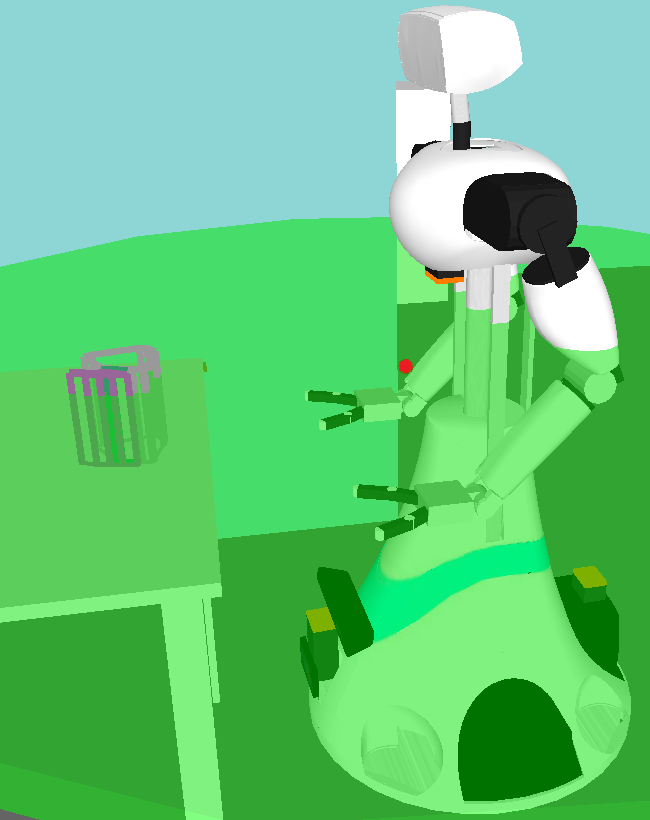
\includegraphics[width = 1\linewidth]{pics/TopologicalHeight_emphsphere}
		\caption{Adjust height grasp: since mainly the height of the end-effector is important, the constraint volume is a cylinder with a large diameter and small height.}
		\label{wbp:fig:topheight}
	\end{subfigure}
	\hfill
	\begin{subfigure}[t]{0.3\linewidth}
		\centering
		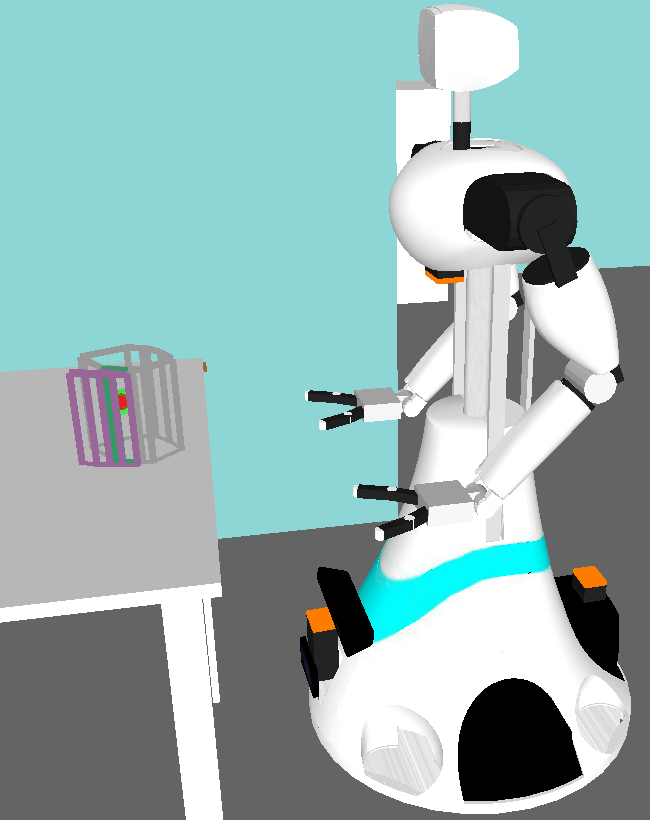
\includegraphics[width = 1\linewidth]{pics/TopologicalGrasp_emphsphere}
		\caption{Grasp: the attractor and constraint volume are inside the wire frame.}
		\label{wbp:fig:topgrasp}
	\end{subfigure}
	\hfill
	\begin{subfigure}[t]{0.3\linewidth}
		\centering
		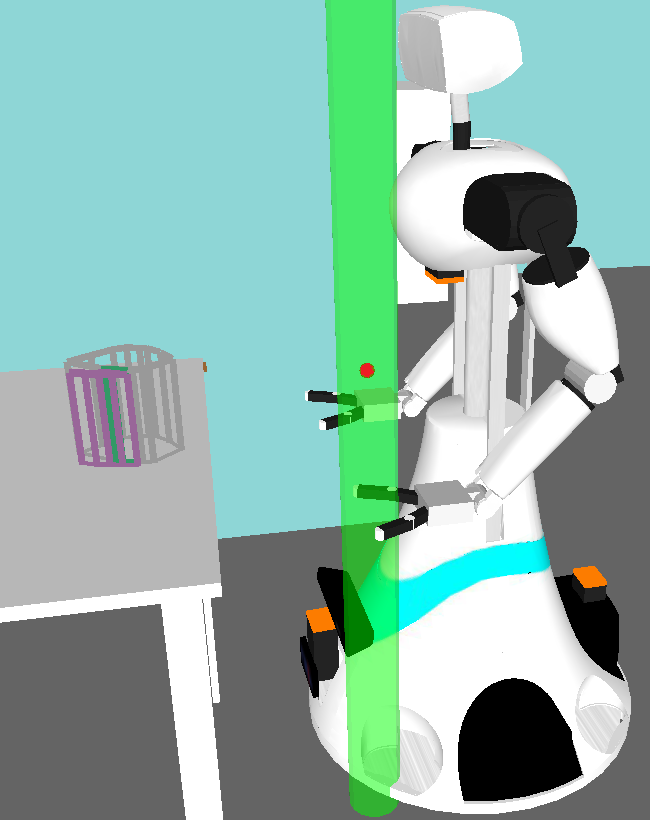
\includegraphics[width = 1\linewidth]{pics/TopologicalRetract_emphsphere}
		\caption{Retracting: since the exact height is irrelevant, the constraint volume is a narrow but tall cylinder.}
		\label{wbp:fig:topretract}
	\end{subfigure}	
	\caption{Visualization of three attractors. The red spheres indicate the exact location of the attractor. The green volume indicates the constraint, \ie, once the end-effector is inside the volume, it can proceed to the next attractor.}
	\label{wbp:fig:constraints}
\end{figure}
All nodes in the graph in Figure~\ref{wbp:fig:constraints} have to be grounded to specific end-effector attractors. Each attractor can constrain up to six \dofs\ and possesses a number of properties:
%Each \dof of a node can be free, \ie, there is no constraint, `static', meaning that the constraint is always the same and `dynamic', meaning that it is updated for every task instance. Obviously, when grasping an object, the \dofs\ are dynamic.
%As mentioned in~\citet{DeSchutter2007}, \emph{at least} two object frames and two feature frames are required to define a constraint.
%Each \dof\ of an attractor can be free or defined with respect to different frames. For example, the end-effector is preferably close to the \emph{robot} when carrying an object, while during a grasping motion the attractor is defined at the object.  
%A number of additional properties must be defined:
\begin{itemize}
    \item Target pose: As mentioned in~\citet{DeSchutter2007}, \emph{at least} two object frames and two feature frames are required to define a constraint.
    The target pose represents the first object frame and the first feature frame. 
	Up to three position and three orientation \dofs\ can be specified.    
%    the position represents up to three position \dofs\ in a specified frame, such that the end-effector is positioned with respect to, \eg, the robot or an object in the environment. Furthermore, the orientation represents up to three orientation \dofs. Again, these can be specified in any frame. 
	\item Target offset:  The target offset represents the second object frame and feature frame. %The problem with having a separate position and orientation constrained is that it is difficult to model possible dependencies between position and orientation. This is, \eg, the case when the end-effector is supposed to move to a pre-grasp pose. Therefore, an additional parameter called target offset is added.
    %represents up to three DoFs in a specified end-effector frame. Together, target position and target offset can define, \eg, pre-grasp constraints: the point straight $15\ \mathrm{cm}$ in front of the end-effector must coincide with
    \item Stiffness: Defines the stiffness of the virtual spring between the current end-effector pose and the desired end-effector pose. If the stiffness is zero, this \dof\ is unconstrained.
    \item Goal tolerance: The position tolerance is currently defined by a box, sphere or cylinder. If the end-effector position is within the position tolerance, the position constraint is met. If a certain \dof\ is free, the tolerance of this \dof\ should be chosen such that it is always met. The orientation tolerance is defined by roll, pitch and yaw tolerance. If the end-effector orientation is within these tolerances, the orientation constraint is met. Again, if a certain \dof\ is free, the tolerance of this \dof\ should be chosen such that it is always met. In case of orientations, $2\pi$ is always sufficient. In the future, it should be possible to define these tolerances in a more flexible way that is not limited to these simple shapes. Furthermore, force tolerances would also be a valuable addition.
\end{itemize}

In Table~\ref{wbp:tab:motions} the \dofs\ that are constrained in case of the motions in Figure~\ref{wbp:fig:graph} are summarized. Furthermore, Figure~\ref{wbp:fig:constraints} shows three examples where specific parameters for the atrractors and tolerances are defined for the AMIGO robot. Here, the attractors in Figure~\ref{wbp:fig:topheight} and Figure~\ref{wbp:fig:topretract} are defined with respect to the robot and the attractor in Figure~\ref{wbp:fig:topgrasp} is inside the object to grasp. 

\subsection{Forward integration}\label{wbp:ssec:feasibility}
By updating the graph based on object to grasp and searching the graph, a sequence of attractors with accompanying stiffness is obtained. Next, it must be validated whether these attractors result in a feasible motion. This is done by forward integration of the closed-loop whole-body controller, similar to~\citet{Behnisch2010}. 

The forward integration simply means the sequence of attractors is fed to a simulator of the system in Figure~\ref{wbp:fig:wbc}. 
As soon as the end-effector meets the specified goal tolerances, the next attractor is fed to the system. If the goal tolerance of one of the attractors is not met after $ni_{\max}$ iterations, this motion is invalidated.
Since the admittance coupling is designed such that the closed-loop position controlled joints are able to track the desired trajectories, $q = q_d$ to speed up the simulation.
%Since the admittance coupling is designed such that the closed-loop position controller is able to track the desired trajectories, the response is sufficiently accurate to validate the feasibility of a motion. Hence, in this simulator, $q = q_d$. 

If the entire sequence of attractors is feasible it is fed to the real robot in exactly the same way. In case a part of the trajectory is not feasible, a possible solution is to repair this interval using a geometric motion planning method such as a probabilistic roadmap~\citep{OBPRM1998,Laumond2000,Kurniawati2004,Yeh2012} or a rapidly exploring random tree~\citep{Hsu1997,Kuffner2000}. This is left as future work.

%\begin{itemize}
%    \item Definition of the grasp: intro to RoboCup, manipulator motions
%    \begin{itemize}
%        \item Refer to Table~\ref{wbp:tab:motions}
%        \item Formerly: in task planner
%        \item Emphasize that this already leads to collision free motions
%    \end{itemize}
%    \item Grounding the nodes: Definition of a constraint
%    \item Free, static, dynamic
%    \begin{itemize}
%        \item Position
%        \item Orientation
%        \item Offset
%        \item Stiffness
%        \item Position constraints
%        \item Orientation constraints
%    \end{itemize}
%    \item Check joint-space feasibility
%    \begin{itemize}
%        \item If not feasible: repair with PRM
%    \end{itemize}
%\end{itemize}

\section{Simulation results}\label{wbp:sec:simulations}
Although the implementation has not yet been finalized, a simulation has been performed to illustrate the approach.
%To demonstrate the use of the topological manipulation planner, a number of simulations and experiments has been performed with the AMIGO robot.
AMIGO is the domestic service robot of the Eindhoven University of Technology. Its base platform has four omniwheels and is hence fully holonomic. It is equipped with two \ndof{7} Philips Experimental Robotic Arms. These have the dimensions of the arms of a large person and are placed on an upper body that can move up and down with a telescopic spine. In its lower position, AMIGO can grasp objects from the floor while in its upper position it has the size of a child and can therefore operate most features in a domestic environment. The kinematic structure of AMIGO is redundant: the two arms and torso have a $2 \times 7 +1 = 15$ \dofs.

In this simulation, AMIGO is performing a typical grasping move. As a comparison, we have also performed this simulation with waypoints constructed in a more common probabilistic roadmap. Here, a visibility-based sampling method~\citep{Laumond2000} has been used in \ndof{6}. The resulting end-effector trajectory can be seen Figure~\ref{wbp:fig:rviz_grasp_global}, while the trajectory of the topological planner is displayed in Figure~\ref{wbp:fig:rviz_grasp_topological}. A striking difference in these trajectories is that the maximum height of the random trajectory equals $1.13\m$, while the actual target is more than $20\cm$ lower at $0.90\m$. As a result, the motion using the PRM planner looks very unnatural and not human-like. Furthermore, the PRM planner does not enforce the end-effector to approach the object to grasp from the correct direction. Finally, the topological planner will always result in a similar trajectory, while a PRM-based planner will result in a different trajectory every time a new roadmap is constructed.
\begin{figure}[ht]
    \begin{subfigure}[t]{0.48\linewidth}
        \centering
        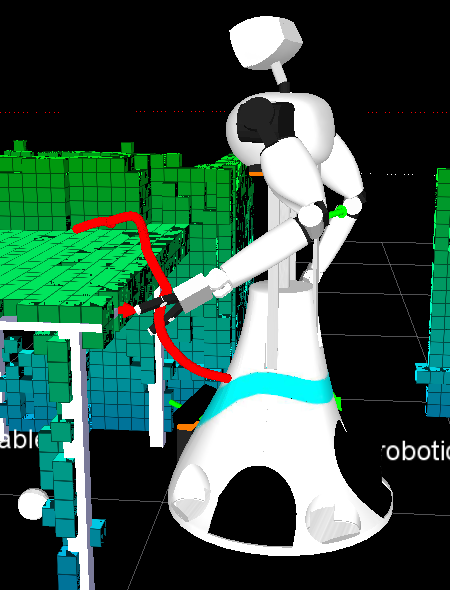
\includegraphics[width = 0.9\linewidth]{pics/Screenshot20140123_144937_crop.png}
        \caption{Using a visibility-based probabilistic roadmap.}
        \label{wbp:fig:rviz_grasp_global}
    \end{subfigure}
    \hfill
    \begin{subfigure}[t]{0.48\linewidth}
        \centering
        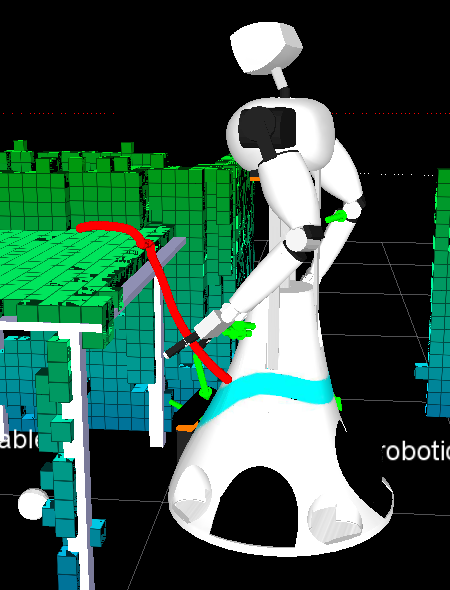
\includegraphics[width = 0.9\linewidth]{pics/Screenshot20140123_145234_crop.png}
        \caption{Using the topological planner.}
        \label{wbp:fig:rviz_grasp_topological}
    \end{subfigure}
    \caption{End-effector trajectories when using a visibility-based probabilistic roadmap and using the topological planner.}
    \label{wbp:fig:rviz_grasp}
\end{figure}
%
%\begin{itemize}
%    \item Planner topological gives more logical motion: does not move to $z = 1.1$. This is a common drawback of planners based on random sampling
%    \item Planner topological gives higher peaks in wrenches (roll, pitch), but is more flat. Difficult to draw a real conclusion out of that
%    \item Torques are way lower
%    \item Norms: squared sum of distances for collision avoidance, resulting torques from cartesian impedance, or the work done by these
%\end{itemize}

\section{Conclusions \& future work}\label{wbp:sec:discussion}
%\begin{enumerate}
%	\item Implementation
%	\item Adding more nodes to the graph
%	\item Currently: position control. Possible extension to force control. 
%	\item Learning
%\end{enumerate}
This chapter demonstrates the use of a topological graph for motion planning for manipulation. Although the implementation of the entire pipeline has not yet been finished, preliminary simulations show promising results. 
A first prerequisite to see the benefits of this planner in practice is to have a decent implementation of the whole-body controller. This allows to make a proper comparison between a geometric planner and a topological planner to assess whether the decreased number of constrained \dofs\ indeed leads to improved performance.
The graph in Figure~\ref{wbp:fig:graph} and Table~\ref{wbp:tab:motions} only contain nodes for simple pick-and-place operations. 
%To make this approach more useful, more nodes should be added to the graph so that more tasks are covered. 
To use this approach in practice, more nodes should be added to the graph so that more tasks are covered. 

As discussed in Section~\ref{wbp:ssec:constraints}, the nodes are grounded using pose constraints. 
%Besides pose constraints, it is very useful to also include force constraints. 
Extending the definition of the attractors, \ie, the grounding of the nodes, offers numerous possibilities to improve performance. One of the possible extensions is to include force constraints.
Consider, for example, the task of placing an object. The `place' move, can then be implemented with the attractor position at the table surface and a force constraint in vertical direction. As a result, the robot will move the object down until it `feels' that it has reached the table. 

\newpage
\section{Appendix A. How to integrate?}

This appendix shows where the whole-body controller and planner are positioned within the TU/e Robotics architecture, depicted in Figure~\ref{app:architecture}. The whole body controller is positioned in the 'Robot skills Implementation' block. The input of the whole body controller is the world model that describes the environment around the robot; as an output, the whole-body controller sends joint references to the low level control or the simulator.
\begin{figure}[ht]
    \centering
    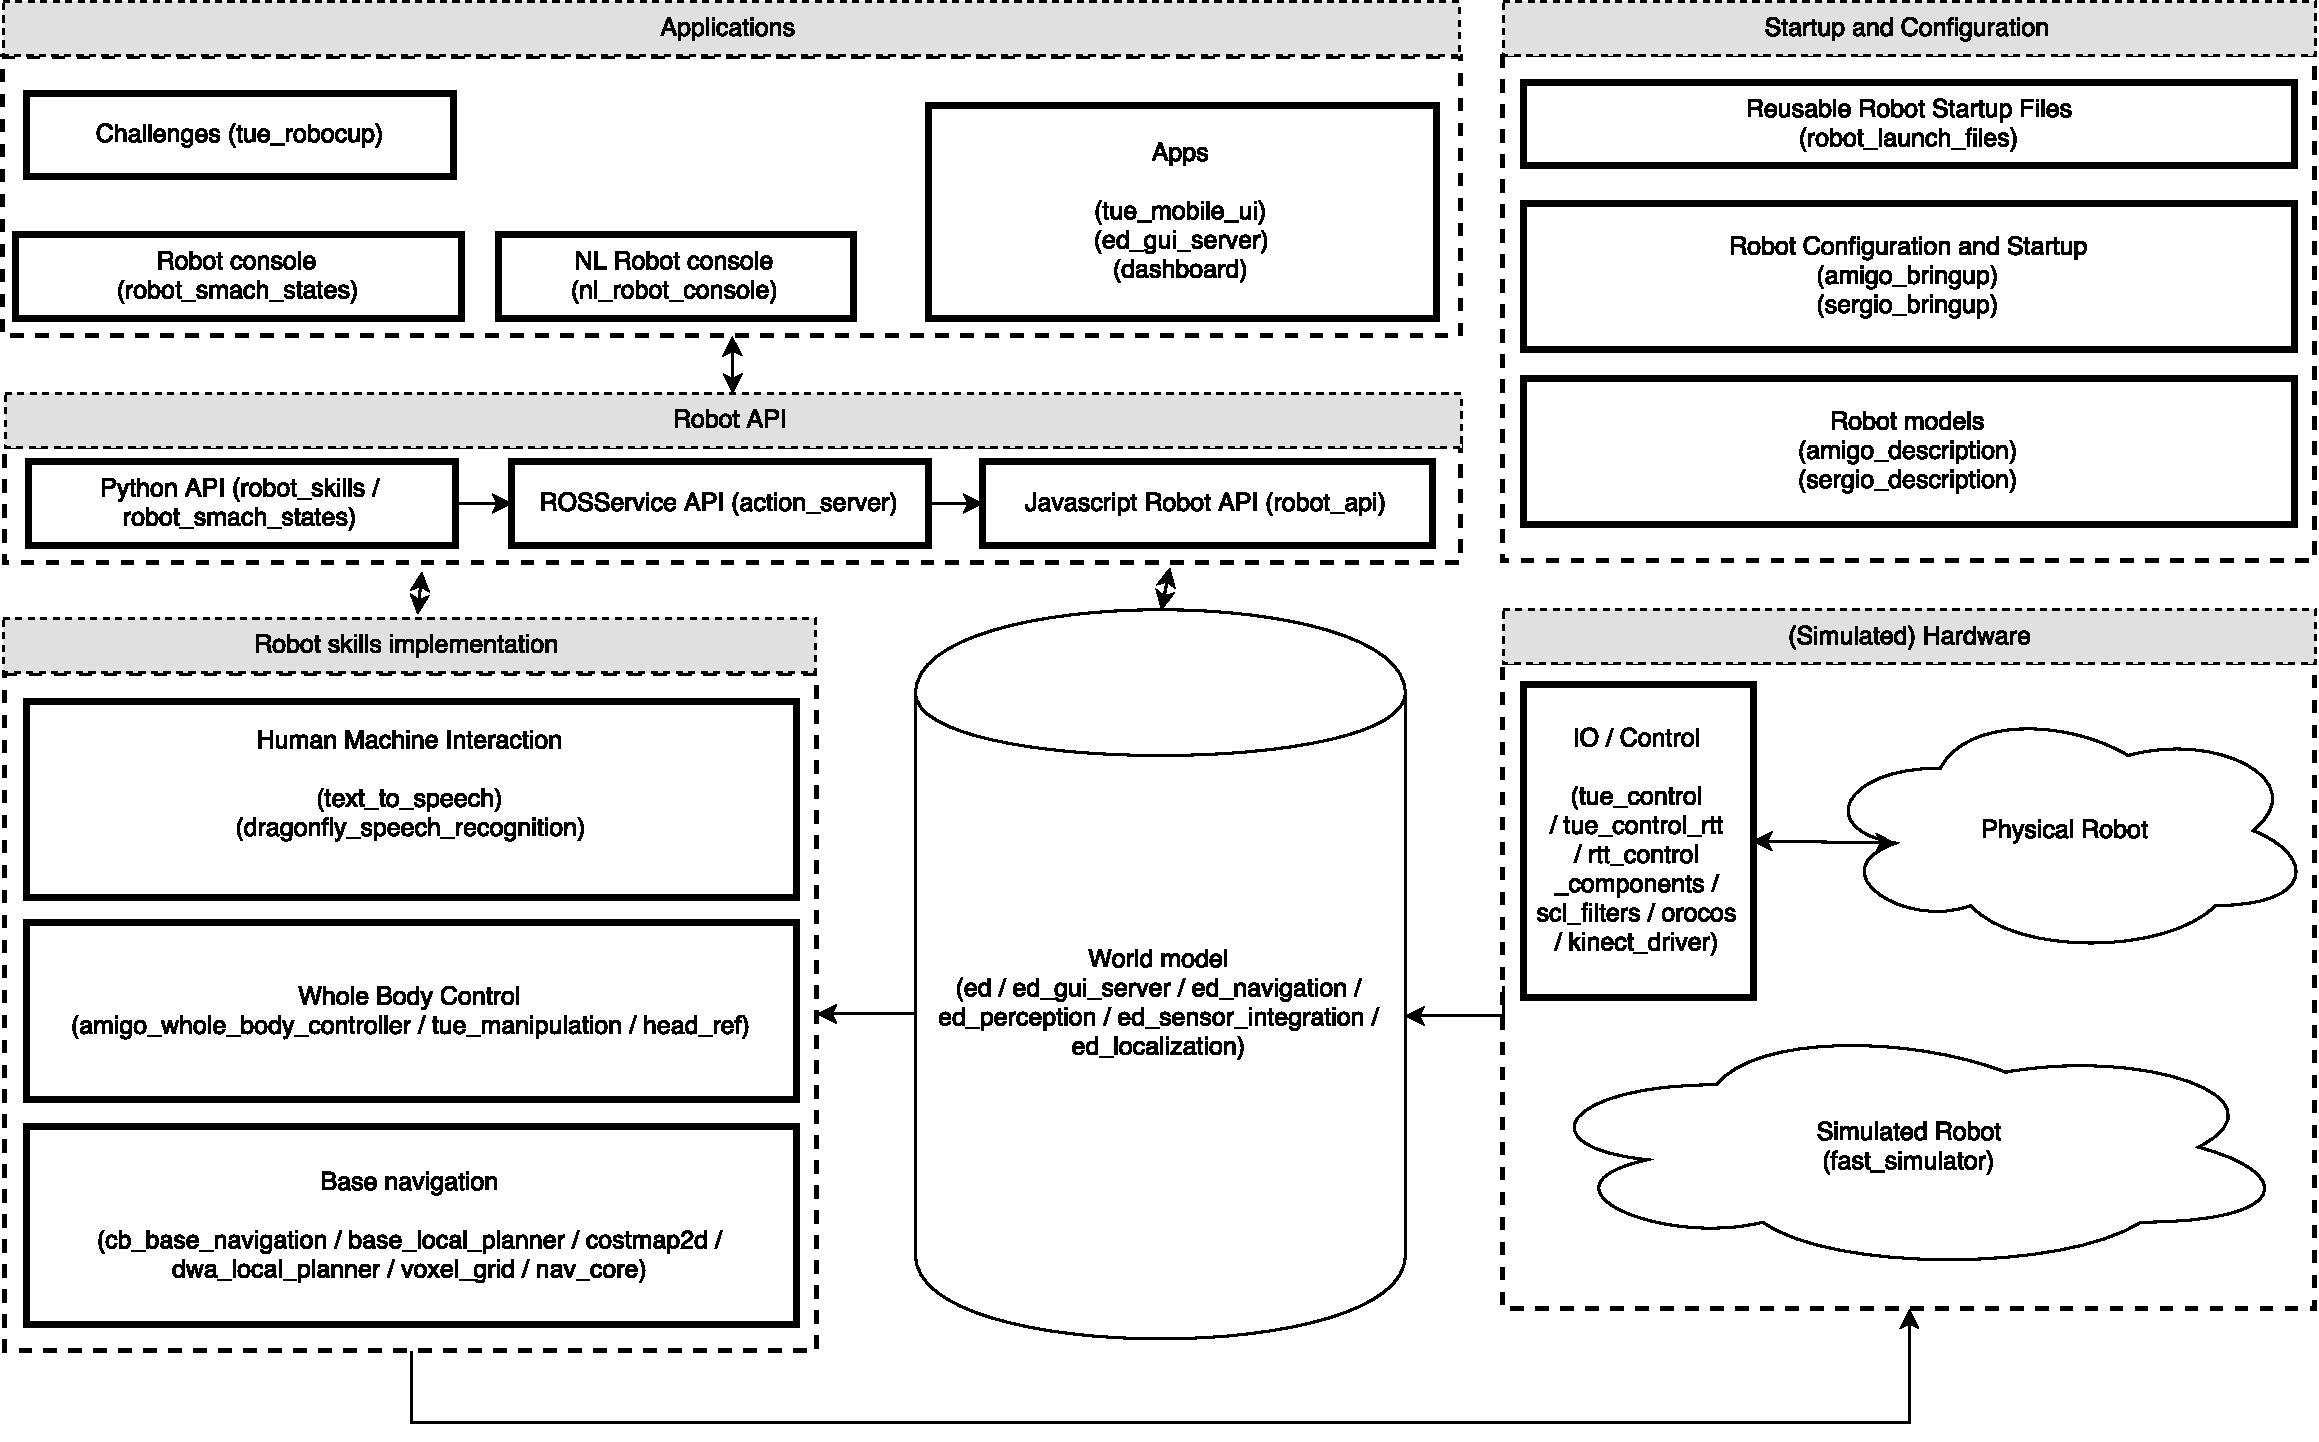
\includegraphics[width = 1.0\linewidth]{pics/architecture.pdf}
    \caption{TU/e Robotics Architecture}
    \label{app:architecture}
\end{figure}
The whole-body controller exposes an API using a ROS actionlib to the Robot API layer so that its functionality can be used as a skill. The actionlib interface definition can be found \href{https://github.com/tue-robotics/amigo_whole_body_controller/blob/master/action/ArmTask.action}{here}; the arguments basically consist of a link name, position constraints and orientation constraints.
\\\\
The output of the whole body controller	are references for the different joints that are taken into account by the controller.
